	\PassOptionsToPackage{brazil,american}{babel}
\documentclass[12pt]{article}

\usepackage{sbc-template}
\usepackage[brazil,american]{babel}
\usepackage[utf8]{inputenc}

\usepackage{graphicx}
\usepackage{url}
\usepackage{float}
\usepackage{listings}	
\usepackage{color}
\usepackage{todonotes}
\usepackage{algorithmic}
\usepackage{algorithm}
\usepackage{hyperref}

\sloppy

\title{Experimento 10\\ 
	CONTADOR SÍNCRONO}

\author{
	Lucas Mafra Chagas, 12/0126443 \\
	Marcelo Giordano Martins Costa de Oliveira,  12/0037301
}


\address{Dep. Ciência da Computação -- Universidade de Brasília (UnB)\\
	CiC 116351 - Circuistos Digitais - Turma C
	\email{\{giordano.marcelo, chagas.lucas.mafra\}@gmail.com}
}

\begin{document}
	
	\maketitle
	
	\begin{abstract}
		In this experiment, we will develop a 3-stage progressive synchronous counter using JK flip-flops.
	\end{abstract}
	
	\begin{resumo} 
		Nesse experimento, iremos desenvolver um contador síncrono progressivo de 3 estágios utilizando flip-flops JK.
	
	\end{resumo}
	
	\section{Objetivos}
	\label{sec:Objetivos}
		Estudo de contadores síncrono e do método de síntese de circuitos sequenciais síncronos, utilizando flip-flops de vários tipos. É feito o projeto e montagem de um contador de 3 estágios com uma certa sequência de contagem, utilizando-se flip-flops JK.
	
	
	\section{Materiais} 
	\label{sec:Materiais}
	
	\begin{itemize}
		\item software Quartus-II
		\item Kit de desenvolvimento DE2 com FPGA Altera Cyclone II.
	\end{itemize}
	
	\section{Introdução}
	\label{sec:Introducao}
	
	Um contador síncrono é um circuito cujos clocks dos flip-flops vêm de uma mesma fonte, ou seja, as entradas de clock de todos os flip-flops estão conectados a uma mesma entrada do circuito.
	Para projetar um contador síncrono, podemos utilizar a tabela de transições do flip-flop JK, que nos diz quais devem ser os valores nas entradas J e K para cada transição de valores na saída quando é dado um pulso de clock.
	Montando a tabela dos valores nas saídas dos flip-flops de acordo com a sequência de pulsos de clock, é possível criar uma tabela de transições de valores para cada uma das saídas. Com estas tabelas de transições, é possível fazer um mapa de Karnaugh para entradas J e K de cada um dos flip-flops, em função das saídas Qi dos mesmos, de modo que podemos projetar o contador síncrono.
	


	\section{Procedimentos}
	\label{sec:Procedimentos}
	
	Foi implementado no Quartus II um contador síncrono progressivo de módulo 6 que conte segundo a sequência abaixo:
	
		\begin{table}[H]
			\centering
			\begin{tabular}{|c|c|c|c|}
				\cline{1-4}
				\multicolumn{1}{|c|}{Sequência} & \multicolumn{1}{|c|}{Q0} & \multicolumn{1}{|c|}{Q1} & \multicolumn{1}{|c|}{Q2}\\
				\hline
				0 & 0 & 0 & 0 \\
				\hline
				1 & 1 & 0 & 0 \\
				\hline
				2 & 0 & 1 & 1 \\
				\hline
				3 & 0 & 1 & 0 \\
				\hline
				4 & 1 & 0 & 1 \\
				\hline
				5 & 1 & 1 & 1 \\
				\hline
			\end{tabular}
		\end{table}
		
		\begin{figure}[H]
			\centering
			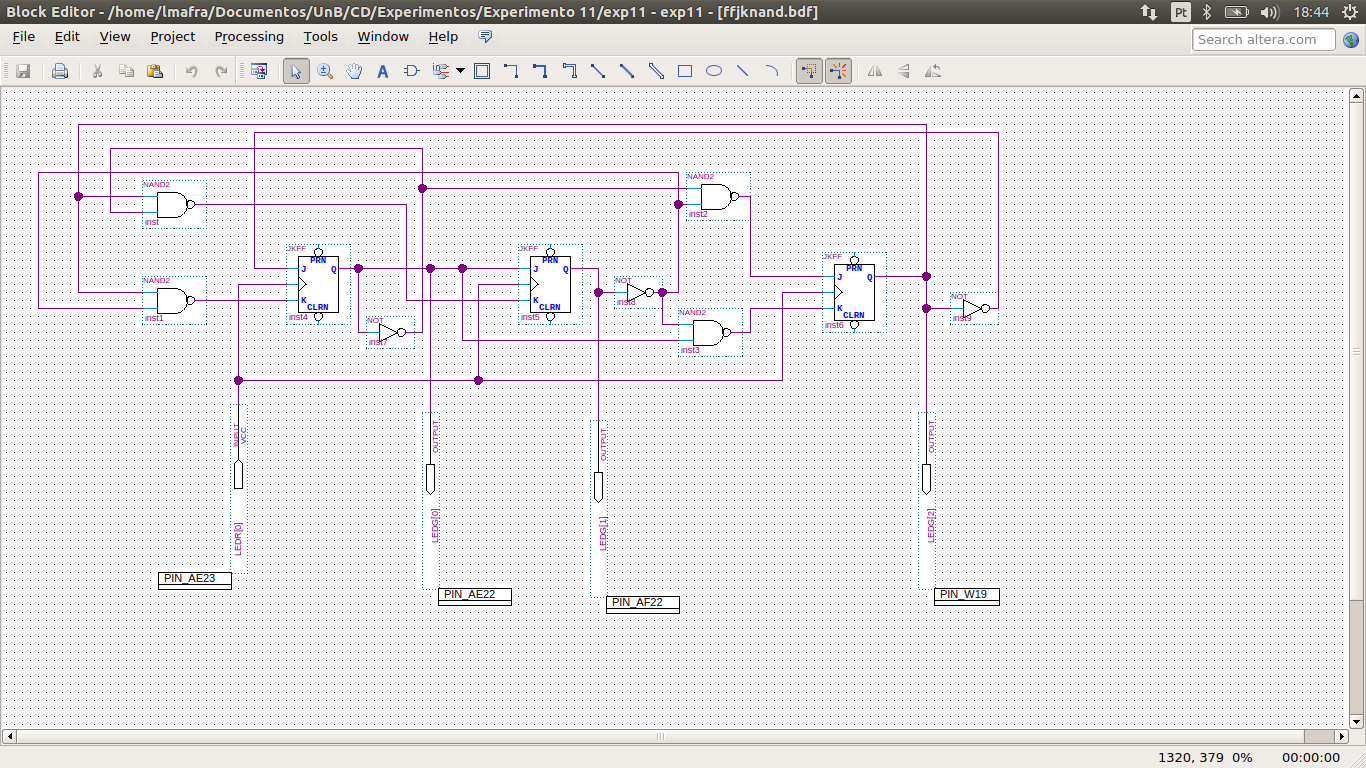
\includegraphics[width=1\textwidth]{contadorsincrono.png}
			\caption{Contador síncrono progressivo de módulo 6 desenvolvido no Quartus II.}
			\label{fig:contadorsincrono}
		\end{figure}
		
		Foi realizado a simulação funcional e temporal do contador.
		
		
		\begin{figure}[H]
			\centering
			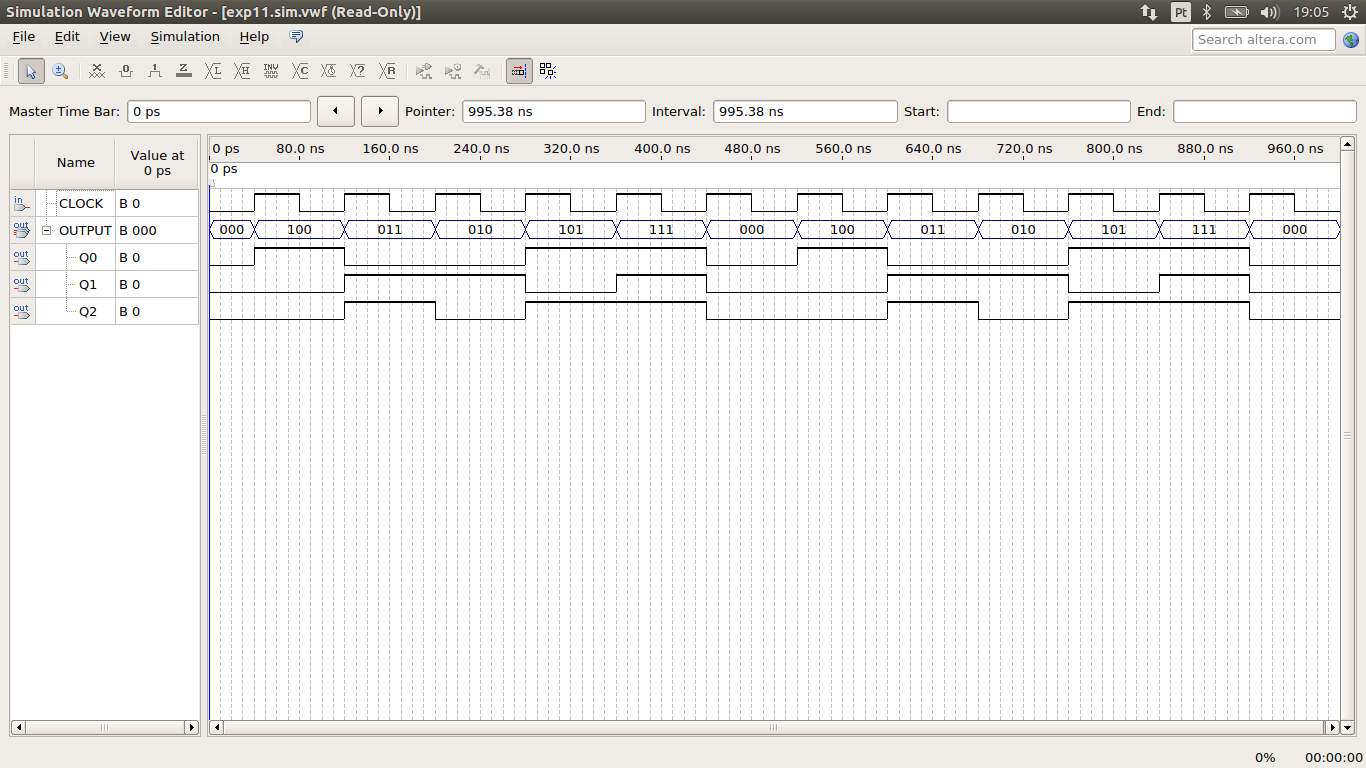
\includegraphics[width=1\textwidth]{simulacaofuncional.png}
			\caption{Simulação funcional do Contador síncrono progressivo de módulo 6.}
			\label{fig:contadorfuncional}
		\end{figure}
		
			\begin{figure}[H]
				\centering
				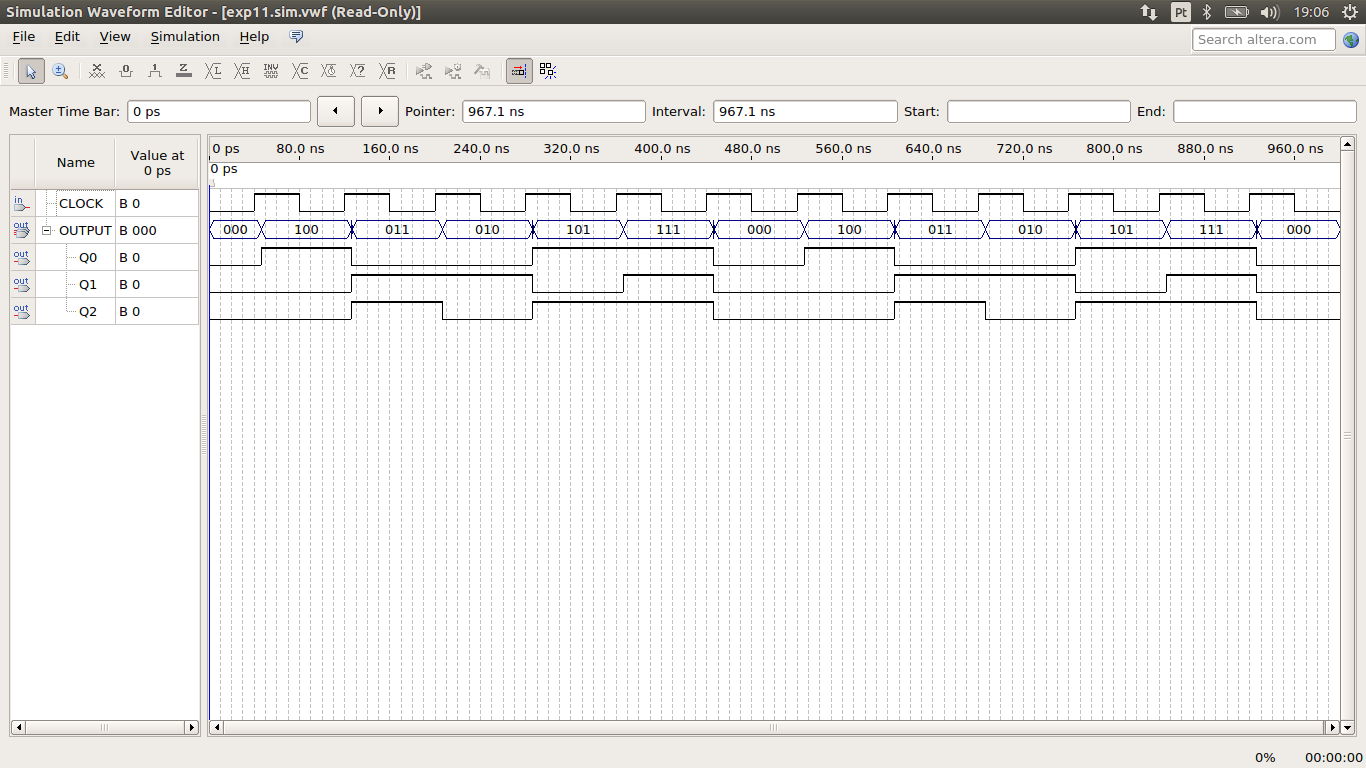
\includegraphics[width=1\textwidth]{simulacaotemporal.png}
				\caption{Simulação temporal do Contador síncrono progressivo de módulo 6.}
				\label{fig:contadortemporal}
			\end{figure}
		
		
		Por fim, sintetizamos o no FPGA do kit de desenvolvimento DE2 e filmamos o seu funcionamento.
		
		É possível ver o resultado no seguinte link: \href{https://youtu.be/lQTI5OIwBo0}{Vídeo no Youtube}.
		
		
	
	\section{Análise dos Resultados}
	\label{sec:Resultados}
	
	
	
	\section{Conclusão}
	\label{sec:Conclusao}
	
	Foi possível perceber o funcionamento dos contadores síncronos, bem como os circuitos sequenciais síncronos, usando flip-flop. Foi possível também perceber a existência de Deadlocks, bem como simplificações do circuito pelo mapa de Karnaugh. O contador com os estados inválidos mostrou que ao acontecer certo erro, o circuito entra em um ciclo infinito de contagem, porém foi devidamente melhorado e arrumado logo após. Enfim, tratou-se de um notável experimento e de um aprendizado maior sobre os contadores.
	
	\newpage 
	% Colocar aqui apenas as respostas dos itens da Auto-Avaliação
	\section*{Auto-Avaliação}
	
	\begin{enumerate}
		\item F
		\item V
		\item V
		\item V
		\item F
		\item F
		\item V
		\item V
		\item F
		\item V
		\item V
		\item F
		\item V
		\item F
		\item V
		\item V
		
	\end{enumerate}
	
	
\end{document}